\subsection{RQ4: an illustrative evidence-window dependence}\label{sec:task-results}
Table~\ref{tab:window-cohort} reports the full-data baselines and calibrated protection across the paired window sizes. Increasing window size improves full-data accuracy before sampling is applied. The healthy-root threshold is \SensitivityThreshold{}\,ms; in the incident mixture it protects about 13\% of traces, making the two smallest tail budgets infeasible. Protection is more frequent in incident windows than in reference windows.

\begin{table}[htbp]
\centering\small
\begin{tabular}{rrrrr}
\toprule
Requests per & Full-data & Full-data & \multicolumn{2}{c}{Protected traces (\%)} \\
window & correct/total & accuracy (\%) & Reference & Incident \\
\midrule
\tableinput{window-cohort-rows.tex}
\bottomrule
\end{tabular}
\caption{The same 600 incidents at three nested window sizes. Protected means root duration at least the calibrated healthy 95th percentile. Each size has its own full-data baseline. All errors remain; the window configurations are dependent.}
\label{tab:window-cohort}
\end{table}

Figure~\ref{fig:window-evidence} connects accuracy to the evidence remaining in each window. At 20\% expected retention with 200 requests per window, head correctly localizes 97.72\% of replay cases and tail 92.68\%, with Monte Carlo standard errors \WindowHeadMCSE{} and \WindowTailMCSE{} percentage points respectively. Head retains about forty requests in each window. Tail retains means of 25.3 reference and 54.2 incident requests. The calibrated rule changes both the allocation of comparison evidence and the retained duration distributions. Prioritizing slow requests can therefore work against this reference-dependent scorer.

\begin{figure}[htbp]
\centering
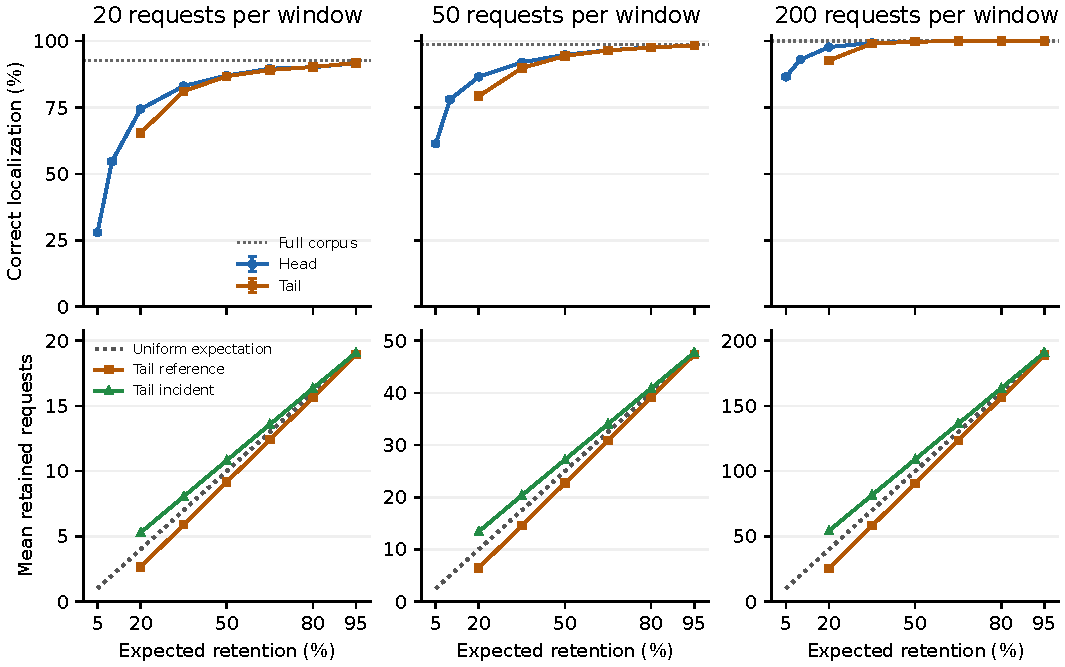
\includegraphics[width=\linewidth]{figures/window-evidence.pdf}
\caption{Illustrative localization on the fixed corpus. Upper panels show replay accuracy with one Monte Carlo standard error, often smaller than the marker; exact full-corpus baselines are dotted. Lower panels show mean retained reference and incident requests under tail; the uniform reference line is the analytical expectation $wp$ for either window. Tail has no feasible points at 5\% or 10\% retention. Lines connect tested rates and do not establish accuracy at intermediate rates.}
\label{fig:window-evidence}
\end{figure}

The dependence concerns both the scorer's baseline and its evidence after selection. At the twenty-request size and 65\% head retention, 260 harmful changes and 139 gains give observed net loss of 2.42 percentage points, with Monte Carlo standard error \WindowNetLossMCSE{} points. The paired calculation includes both outcomes. Increasing replay trials can reduce this simulation uncertainty, but adds no observed incidents. Complete configurations, losses, gains, abstentions, retained counts, and descriptive strata remain in the artifact.
